\documentclass{article} % For LaTeX2e
\usepackage{nips12submit_e,times}
\usepackage{natbib}
\usepackage[pdftex]{graphicx}
%\documentstyle[nips12submit_09,times,art10]{article} % For LaTeX 2.09


\title{Binary Separation on Heterogeneous Image}

\author{
Fisher Yu \\
\texttt{fy@princeton.edu}
\And
Nanxi Kang \\
\texttt{nkang@princeton.edu} 
\And
Siyu Liu\\
\texttt{siyuliu@princeton.edu}
}

\newcommand{\fix}{\marginpar{FIX}}
\newcommand{\new}{\marginpar{NEW}}

\nipsfinalcopy % Uncomment for camera-ready version

\begin{document}


\maketitle

\section{Introduction}

In computer vision, image segmentation is a process of partitioning an 
image into several pixel groups. The pixels in each group should have 
something in common, such as color, intensity or texture. The goal
 of image segmentation is to change the representation of an image into
 something meaningful and easy to understand. It is typically
 used to locate objects and boundaries in an image. An interesting 
application of image segmentation is to track facial features or objects
 of significance in a performance-driven animation. This helps to 
better compress the animation without loss of important information.

Particularly, how to partition an image into two segments: ``foreground''
 and ``background'' is of special interest. Earlier techniques focused 
on finding the boundary curves between the objects and background. 
The algorithms include snakes~\citep{Kass1988snakes}, active 
contours~\citep{Isard1998condensation}, geodesic active
 contours~\citep{Caselles1995geodesic} and so on. A recent new approach 
by~\citet{Boykov2006graph} demonstrates new potential for solving 
this problem. The approach relies on some manual sketchy on the original
 image. To be specific, a user draws a few red strokes in the foreground 
objects and a few blue ones in the background. Therefore, the algorithm
solves image segmentation based on some extra knowledge about the
 background and foreground. However, one obvious problem with this approach 
is that it requires additional manual efforts, which limits the number 
of images that can be processed. Moreover, as the strokes are roughly
drawn, it introduces some uncertain errors when the boundary between 
``foreground'' and ``background'' is not quite distingushiable.

In this project, we propose a new approach to partition ``foreground''
and ``background'' based on distance data about real objects in the image.
For each image to be processed, we have additional data telling the 
distances between the camera and the objects in real corresponding to some
 pixels in the image. To be specific, when an image is taken by camera, 
there is a one-to-one mapping from pixels in the image to real objects. 
And the additional data tells distance between camera and some real objects 
corresponding to certain pixels in the image. Therefore, we have some 
prior knowledge about how far are some pixels in the image to the camera.

The information can help us analyze whether a pixel belongs to ``foreground'' 
or ``background''. But this information is not complete, as it only covers 
very few pixels. Moreover, it may contain some errors. For example, some pixel
may be mapped to a wrong real object resulting in a wrong distance number.
As the distance data is not quite reliable, we plan to only use it to generate 
the initial states of pixels, i.e, whether it belongs to ``foreground'' or not.
Based on the inital states, we'll iteratively refine the segmentation following 
the traditional Expectation Maximization process. To do the refinement, we'll 
use Markov Random Fields to calculate the log-likelihood of a pixel, taking the
information of the 8 pixels around it into account.

We believe our approach is more accurate than previous work. The additional 
distance data is a good indicator about the which group a pixel belongs to, 
thus giving us confidence in the accuracy of segmentation, compared to earlier
 techniques which only use the image information alone. Moreover, our approach is 
flexible in that it does not need manual annotation. Finally, the approach
is not likely to be misled by the errors in distance data, since it will do 
iterative refinement based on the pixel's local neighbor information.



\section{Data}
We got our data from Google street view team and processed it to use
the images in our project. The data was collected by a car equiped
with 8 cameras and 3 laser scanners. Each of the laser scanner can scan 180 degree 2D
plane at each time. Two of the laser scanners scanned vertically and
the third one scanned horizontally. As the car moved, the car
positions were recored by global positioning system. Those positions
were adjusted by the scans of the horizontal laser scanner using SLAM
(Simultaneous localization and mapping) techniques to get the best
precision. The 3D position of each laser scan point can be
estimated based on the relative position between the car and laser
scanners and therefore a 3D point cloud can be built from the scans of
the vertical laser scanners. At the same time, the eight
cameras were taking pictures as the car moved. Although the cameras
were well calibrated, the images were taken by rolling shutters and
there are errors in terms of image projection model if we assume each
image were taken in a pinhole model.

Given the 3D point cloud and images, we project the points into the
images with the estimated point positions, camera poses and projection
matrices. Then we can get images like Figure~\ref{fig-data_image}.

\begin{figure}[h]
\begin{center}
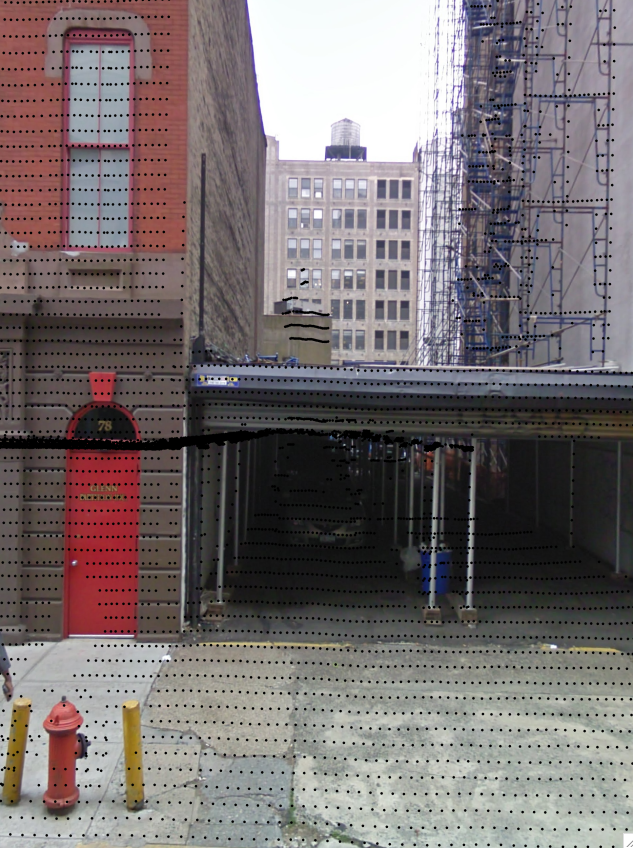
\includegraphics[height=0.5\linewidth]{./fig/image_sample.png}
\end{center}
\caption{An image with 3D points projected into it.}
\label{fig-data_image}
\end{figure}

In Figure~\ref{fig-data_image}, the black dots are the projections of
the 3D points in this image. As you can see, due to all kinds of
errors mentioned above, the 3D projections and the images are not well
aligned and we can't segment the images directly based on the depth of
the 3D scan points. In this project, we want to find the contour
between the background (the sky area) and foreground (all the objects
appears in the image, including roads and buildings). The models and
computing issue will be discussed in the methods section.

\section{Methods}

We propose to formulate the background and foreground separation
problem as labeling problem. We assign each pixel a binary latent
variable representing the category of the pixel. For each
segmentation (foreground or background), we plan to use Gaussian Mixture Model to model the
distribution of the colors. If the distribution of the pixel colors
are independent, we can use the mixture model together with EM
(Expectation-Maximization) algorithm to solve the assignment of labels
directly. However, this method would not work well because we would
get very noisy label assignment to the pixels. The essential problem
is that there is interaction between adjacent pixels. If all the
neighbors of a pixel are labeled foreground, it is more possible that
this pixel also belongs to foreground. We plan to
use MRF(Markov Random Field) to model this idea. As mentioned in
introduction, this model is widely used by a lot of works. A good
survey is in~\citep{Szeliski2008Comparative}.

\begin{figure}[ht]
\begin{center}
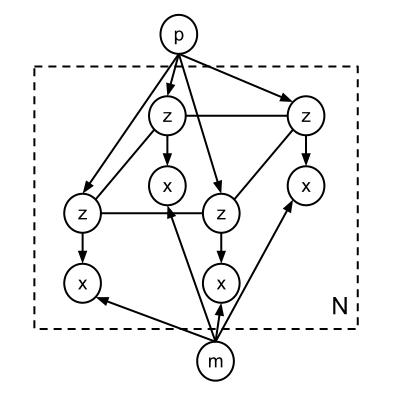
\includegraphics[height=0.5\linewidth]{./fig/graphical_model.png}
\end{center}
\caption{The model we proposed.  $x$ are the values of the
pixels. $z$ are the latent labels of each pixel. $p$ is the parameter
for $z$ and $m$ is the parameter for the Gausian Mixture Model.}
\label{fig-graphical_model}
\end{figure}

The graphical representation of our model is shown in
Figure~\ref{fig-graphical_model}. $x$ are the values of the
pixels. $z$ are the latent labels of each pixel. $p$ is the parameter
for $z$ and $m$ is the parameter for the Gausian Mixture Model. We
plan to use EM algorithm for the inference. In the M step, the model
parameters can be got by maximum likelihood. In the E step, it is
actually hard to get an exact posterior distribution for the latent
labels because the latent variables are not independent. So to solve
this MRF model, we plan to try several approximate inference methods
on MRF such as~\citep{Boykov2006graph}.

\section{Evaluation}
As explained before, the goal for this project is to separate the forground from background in street view images. However, provided ground truth is not available in our dataset, directly measuring the error seems not feasible (though we can measure the enery in the resulting MRF but it might not corresponding to the optimal behaviors as pointed out in~\citet{Szeliski2008Comparative}). Thus, we plan to do a series of comparative expriments with current interactive methods mentioned in~\citep{Szeliski2008Comparative}. Although modern MRF-based segmentation algorithms performs reasonably well, human facilitations during the process might be less favored in large dataset such as the street view dataset. Therefore,  by taking advantage of the LiDAR inputs, we are hoping to use sparse depth information as guidence to develop an automatic alternative yet competitive approach for binary image segmentation task. If our algorithm works as our optimistic estimation, we would attempt to generalize it into segmentation for multiple objects upon which we could further use these segments for image matching and possibly build models for 3D meshes for different objects accordingly. On the other hand, if the proposed method could not meet our expectation, we would like to explore the possibilities of reorganizing our lidar data as proper inputs for the interactive methods as in~\citep{Rother2004GrabCut} and~\citep{Arbelaez2011Contour}.

\bibliography{proposal}
\bibliographystyle{abbrvnat}


\end{document}
